\documentclass[border=4pt]{standalone}
% Shared style for every diagram. Colour-blind-safe palette (Okabe-Ito).
\usepackage[T1]{fontenc}
\usepackage{helvet}
\renewcommand{\familydefault}{\sfdefault}
\usepackage{tikz}
\usetikzlibrary{arrows.meta,positioning,fit,backgrounds,calc,shapes.geometric,decorations.pathreplacing}
\definecolor{cblue}{HTML}{0072B2}
\definecolor{corange}{HTML}{E69F00}
\definecolor{cgreen}{HTML}{009E73}
\definecolor{cred}{HTML}{D55E00}
\definecolor{cpurple}{HTML}{CC79A7}
\definecolor{cgrey}{HTML}{6B7280}
\definecolor{csky}{HTML}{56B4E9}
\tikzset{
  >={Stealth[length=2.2mm]},
  box/.style={draw, rounded corners=3pt, align=center, minimum height=11mm, minimum width=22mm, font=\small, line width=0.7pt},
  real/.style={box, draw=cblue, fill=cblue!8},
  sim/.style={box, draw=corange, fill=corange!12},
  future/.style={box, draw=cgrey, dashed, fill=white},
  flow/.style={->, line width=0.8pt, draw=black!75},
  dflow/.style={->, line width=0.8pt, dashed, draw=cgrey},
  lbl/.style={font=\scriptsize, text=black!70},
  group/.style={draw=black!25, rounded corners=6pt, inner sep=6pt},
}

\begin{document}
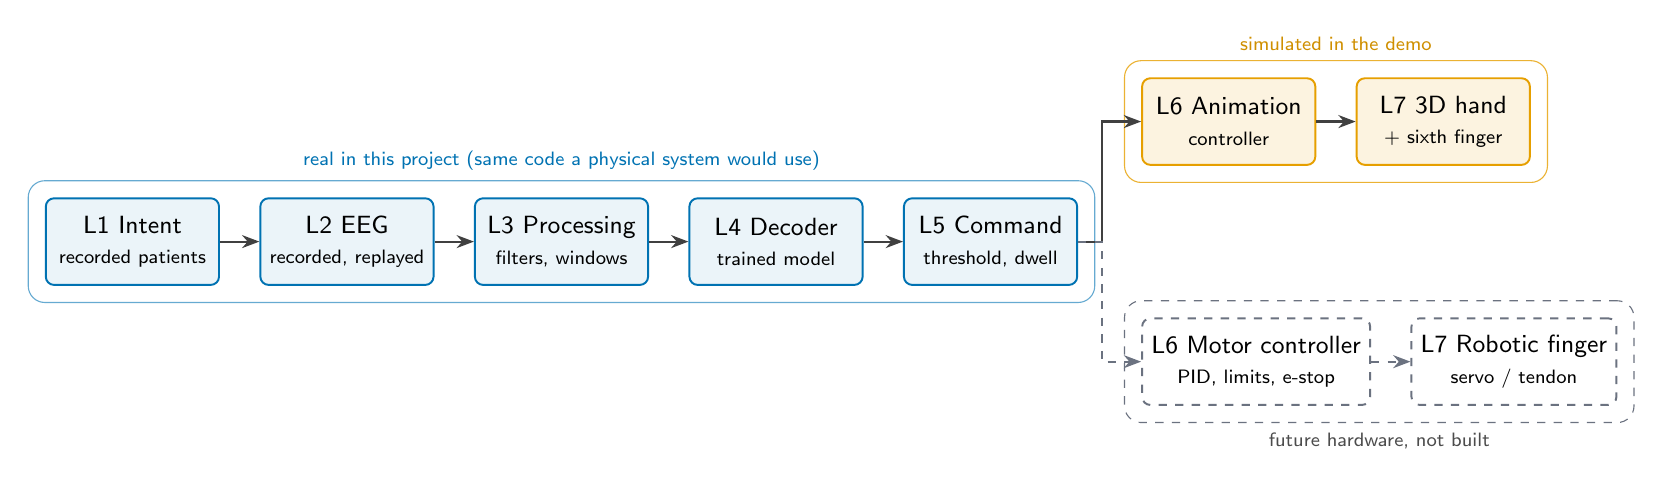
\begin{tikzpicture}[node distance=5mm]
  \node[real] (l1) {L1 Intent\\\scriptsize recorded patients};
  \node[real, right=of l1] (l2) {L2 EEG\\\scriptsize recorded, replayed};
  \node[real, right=of l2] (l3) {L3 Processing\\\scriptsize filters, windows};
  \node[real, right=of l3] (l4) {L4 Decoder\\\scriptsize trained model};
  \node[real, right=of l4] (l5) {L5 Command\\\scriptsize threshold, dwell};
  \foreach \a/\b in {l1/l2, l2/l3, l3/l4, l4/l5} \draw[flow] (\a) -- (\b);
  \node[sim, above right=4mm and 8mm of l5] (l6s) {L6 Animation\\\scriptsize controller};
  \node[sim, right=of l6s] (l7s) {L7 3D hand\\\scriptsize + sixth finger};
  \node[future, below right=4mm and 8mm of l5] (l6r) {L6 Motor controller\\\scriptsize PID, limits, e-stop};
  \node[future, right=of l6r] (l7r) {L7 Robotic finger\\\scriptsize servo / tendon};
  \draw[flow] (l5.east) -- ++(3mm,0) |- (l6s.west);
  \draw[dflow] (l5.east) -- ++(3mm,0) |- (l6r.west);
  \draw[flow] (l6s) -- (l7s);
  \draw[dflow] (l6r) -- (l7r);
  \begin{scope}[on background layer]
    \node[group, draw=cblue!60, fit=(l1)(l5), label={[lbl, text=cblue]above:real in this project (same code a physical system would use)}] {};
    \node[group, draw=corange!80, fit=(l6s)(l7s), label={[lbl, text=corange!90!black]above:simulated in the demo}] {};
    \node[group, draw=cgrey, dashed, fit=(l6r)(l7r), label={[lbl]below:future hardware, not built}] {};
  \end{scope}
\end{tikzpicture}
\end{document}
